
\documentclass[a4paper,fleqn]{tufte-handout} 
\usepackage{graphicx} 
\usepackage{morefloats,textcomp} 
\usepackage{amsmath} 
\usepackage{amssymb} 
\usepackage{rotating,url} 
\definecolor{violet}{rgb}{0.8, 0.6, 0.8}
\definecolor{green}{rgb}{0.8 ,.9, 0.8}
\definecolor{blue}{rgb}{0.3, 0 ,0.6}
\usepackage[]{hyperref}
% mcode options for matlab code insertion bw (for printing), numbered (line numbers), framed (frame around code blocks), useliterate (convert Matlab expressions to Latex ones), autolinebreaks (automatic code wraping, use it with caution 
\usepackage[useliterate]{mcode} 
\graphicspath{{figures/}{report/figures/}{../figures/}{../../}}  

\title{ expLanes: beautiful computational experiments } 
\author{ Mathieu Lagrange } 

\newcommand{\explanes}{\textsf{expLanes} }  

\lstset{aboveskip=2pt,belowskip=2pt, basicstyle=\small} % \medskipamount

\begin{document} 
  
\maketitle 

\section{About you}

Let's assume that you are practicing computational experiments. Most probably, this takes you time and a lot of care, and may be you have some frustrations depending whether you are:
\begin{itemize}
\item  \textbf{a Master's student ?} Then, you may at some point consider the fact that the problem is not simply to come with a new idea and implement it. To contribute significantly to the research community are striving to be part of, you need to compare your method with the ones of others. This process is tedious, hard if not impossible and involve a lot of coding and knowledge about large scale data processing, statistical analysis and reporting of quantitative data.

\item \textbf{a PhD student ?} You have several years to dedicate to a research project. Doing it well will help you stay motivated and efficient. But how ? Several years of work means a lot of code, a lot of bugs, a lot of failures and hopefully some gain of knowledge for you and your research community. How will you keep track of those many experiments ? How will you efficiently document them ?  How will you quickly report your progress to the members of your research team ? How will you publish your research in a reproducible way ?

\item \textbf{a Post doctoral fellow ?} You are now an established researcher, with many ideas about what could be done in order increase knowledge in your community. But you also have to juggle with many different projects you are involved in. Keeping track of all those projects and being able to easily switch between them is mandatory for success. For example, being able to re-run years old experiments in order to efficiently satisfy a reviewer request is critical for your career.

\item \textbf{a Full time researcher ?} Besides research, you have many duties that shreds the time you can allocate to pursue the many personal research projects you have. The time needed to switch between several projects is sometimes too long with respect to the time you can allocate to reach efficiency. More importantly, the free time you have is usually not in front of your desktop. Also, you are advising several students and most of the time, when the student goes away, the project ends at best with a student specific organization of code and data that will most probably not help the next student to pursue efficiently the research project you are interested in.

\end{itemize}

And for all or others, you are heading towards sharing your code but you are not confident with your programming expertise and you do not have time to improve your experimental code into a sharable state\footnote{\url{http://sciencecodemanifesto.org}} ?

If so, please consider giving \explanes a try as it is specifically designed with those matters in mind and hopefully will help you reducing specific burden that keep you way from reaching this goal which is one of the most important step towards true expansion of knowledge in science and engineering: reproducibility\cite{science, sp}.

\section{Features}

\explanes is a software framework currently implemented in Matlab that 
\begin{itemize}
\item provides a high level abstraction for running computational experiments
\item allows multiple users per experiment
\item allows multiple processing platforms to be used
\item features an strong decoupling of 3 major experimental phases: 
\begin{enumerate}
\item coding
\item processing
\item reduction of results.
\end{enumerate}
\end{itemize}

\section{Benefits} 
\begin{enumerate}
\item The user can focus on solution code,
\item evaluated with standard experimental designs.
\item Bugs and the time needed to solve them is reduced,
\item context switching between projects is much easier
\item as well as diffusion of reproducible code.
\end{enumerate}

\section{The scientific method}

The scientific method is a well established method to gain knowledge with demonstrated merit. Sadly, modern ways of doing research impose strong pressure on the time and efforts that can be allocated to a project. The consequence is that important steps of the scientific are often neglected. 

We believe that this quest for speed adversely reduces the meaningfulness of the research results that are nowadays published. Admittedly though, following strictly the scientific method can be tedious and shortcuts might be tempting. \explanes is designed to assist you in the most tedious and most error prone steps and will hopefully help you dedicate more time to the fundamental steps of the scientific method.

Quickly put, the scientific method can be divided into several steps that each may have to be iterated. On the following table, we stated where the \explanes framework can be helpful during this iteration process.

\begin{center} \bf The scientific method\cite{right} \end{center}
\begin{tabular}{clc}
\bf Phases & Steps  & \explanes \\
\hline
\bf Analysis & Describe problem & \\
& Set performance criteria & \\
& Investigate related work & \\
& State objective & \\
\bf Hypothesis & Specify solution & \\
& Set goals & \\
& Define factors & + \\
& Postulate performance metrics & + \\
\bf Synthesis & Implement solution & ++ \\
& Design experiments & +++ \\
& Conduct experiments & ++++ \\
& Reduce results & +++ \\
\bf Validation & Compute performance & ++ \\
& Draw conclusions & +\\
& Prepare documentation & + \\
& Solicit peer review & \\
\end{tabular}

\section{Installation}

\explanes operates in the Matlab environment. A recent version of this software (> R2014) is needed as well as the Statistical toolbox. The Parallel toolbox is needed for in session multi-core processing. 

As much as possible, \explanes uses built in tools to manipulate data. However some functionality are handled through the use basic Unix tools:
\begin{enumerate}
\item \textbf{pdflatex}: handles compilation of reports written in \LaTeX.
\item \textbf{rsync}: allow backup, generation of bundles and data communication between hosts.
\item \textbf{ssh}: allow secure connection between host.
\item \textbf{screen}: allow handling of several detached terminals for background processing.
\end{enumerate}
Please note that those tools must be available on every host where an \explanes project is processed. That said, \explanes do not enforce their availability. For example, without \mcode{pdflatex}, no reports can be generated.

Probing access of those tools by your \explanes project (in this documentation, the project we will demonstrate is called \mcode{geometricShape}) can be done using the following command:

\mcode{geometricShape('probe', 1);}

It also check if the different data paths and processing hosts are achievable. Each of those configuration parameters can be set for each user by editing the configuration file of the project. A default configuration file that is used as template when creating a new project is available at \texttt{$\sim$/.expLanes/<userName>Config.txt}.

\subsection{Linux}

On Linux hosts, the installation should be straightforward. For example, on Debian, Ubuntu systems, the following packages should be sufficient:

\mcode{texlive-full rsync openssh-server openssh-client screen}

Installation may be achieved by typing in a terminal: 

\mcode{sudo apt-get install <packagesNames>}

Minimal configuration might be needed to configure ssh on client and server sides depending on your network configuration. In \explanes ease of use is achieved by using empty passphrase logging.

\subsection{Mac OS}

Several alternatives are available to install Unix packages: Fink, MacPorts and Homebrew. You shall avoid the use of \mcode{/usr} for installation, and the \mcode{PATH} environment variable shall be properly set.

\subsection{Windows}

For pdflatex, please use MiKTeX, for the remaining please use Cygwin. Some tweaks might be needed in order to ensure that the paths and usernames are correct.

\section{\explanes in a nutshell}

\explanes is designed to provide you with as stream lined set of tools to efficiently build the computational environment you need in order to gain knowledge about a research statement.

For the sake of simplicity, we will now consider a trivial research statement. We want to gain knowledge about the base area and the volume of a few 3 dimensional geometrical shapes. For reference, this project is available in the \mcode{demonstrations} directory. %

First, we assume that the \explanes framework is in your path, if not, please type the following in your command window: \\ \mcode{addpath(genpath('<pathToExplanes>'));};

\subsection{Create project}

Let us call create the project \textsl{geometricShape}:
\mcode{expCreate('geometricShape');}
The command ends by moving into the experiment directory.

\subsection{Define steps}

The processing steps can be now be instantiated:

\mcode{geometricShape('addStep', 'base');}

\mcode{geometricShape('addStep', 'space');}

\noindent
Alternatively, the  3 previous commands can be operated at once: \\
\mcode{expCreate('geometricShape', \{'base', 'space'\});}


\subsection{Define factors}

We are interested in the potential impact of the different attributes (shape, color, radius, width, height) of the geometric shape on its base area and volume. The shape can be a cylinder a pyramid or a cube:
\begin{lstlisting}
geometricShape('addFactor', ...
	{'shape', {'cylinder', 'pyramid', 'cube'}});
\end{lstlisting}
The shape can be blue or red:
\begin{lstlisting}
geometricShape('addFactor', {'color', {'blue', 'red'}});
\end{lstlisting}
The radius of the cylinder (modality 1 of factor 1) can be 2, 4, or 6 meters:
\begin{lstlisting}
geometricShape('addFactor', {'radius', '[2, 4, 6]', '', '1/1'});
\end{lstlisting}
The width of the pyramid and the cube (modalities 2 and 3 of factor 1) ranges from 1 to 3 meters:
\begin{lstlisting}
geometricShape('addFactor', {'width', '1:3', '', '1/[2 3]'});
\end{lstlisting}
The height of the shape is only relevant for processing step 2 and for the cylinder of the pyramid (modalities 2 and 3 of factor 1):
\begin{lstlisting}
geometricShape('addFactor', {'height', '2:2:6', '2', '1/[1 2]'});
\end{lstlisting}


Factors can be viewed by typing: \mcode{<experimentName>();}, thus \mcode{geometricShape();} now returns:
\begin{lstlisting}
Factors:
1    shape =  =  = {'cylinder', 'pyramid', 'cube'}
2    color =  =  = {'blue', 'red'}
3    radius =  = 1/1 = [2, 4, 6]
4    width =  = 1/[2 3] = 1:3
5    height = 2 = 1/[1 2] = 2:2:6
\end{lstlisting}
The factors can be edited in the file \\ \mcode{<shortExperimentName>Factors.txt}, that is \mcode{geshFactors.txt}. A setting is a set of modalities, one of each factor of interest.

\subsection{Implement processing steps}

The first step is dedicated to the computation of the base area of the shape. The solution code is implemented in \mcode{gesh1base.m}:
\lstinputlisting[firstline=16, lastline=23]{../demo/geometricShape/gesh1base.m}
We assume here that $\pi$ is known up to a given precision, but 100 measurements have been made.

The second step build on the result of the first processing step to compute the volume (implemented in \mcode{gesh2volume.m}):
\lstinputlisting[firstline=16, lastline=23]{../demo/geometricShape/gesh2space.m}

\subsection{Define observations}

Observations for the 2 processing steps are the following. First step:
\lstinputlisting[firstline=24, lastline=24]{../demo/geometricShape/gesh1base.m}
Second step:
\lstinputlisting[firstline=25, lastline=26]{../demo/geometricShape/gesh2space.m}

\begin{marginfigure}
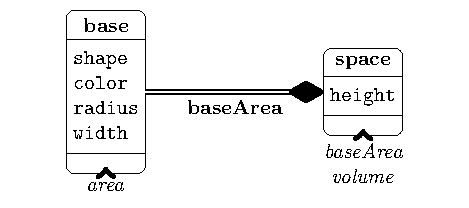
\includegraphics[width=1.2\textwidth]{../demo/geometricShape/report/figures/factors}
\end{marginfigure}

The command \mcode{geometricShape('f')} generates a diagram view of the experiment.

\subsection{Process}

\begin{lstlisting}
geometricShape('do', 1);
\end{lstlisting}
run the base step over all 18 settings.
\begin{lstlisting}
geometricShape('do', 0, 'mask', {[1 2] 0 1});
\end{lstlisting}
runs successively every steps over the cylinders of radius 2  and all the pyramids.

\subsection{Expose observations}

\begin{marginfigure}
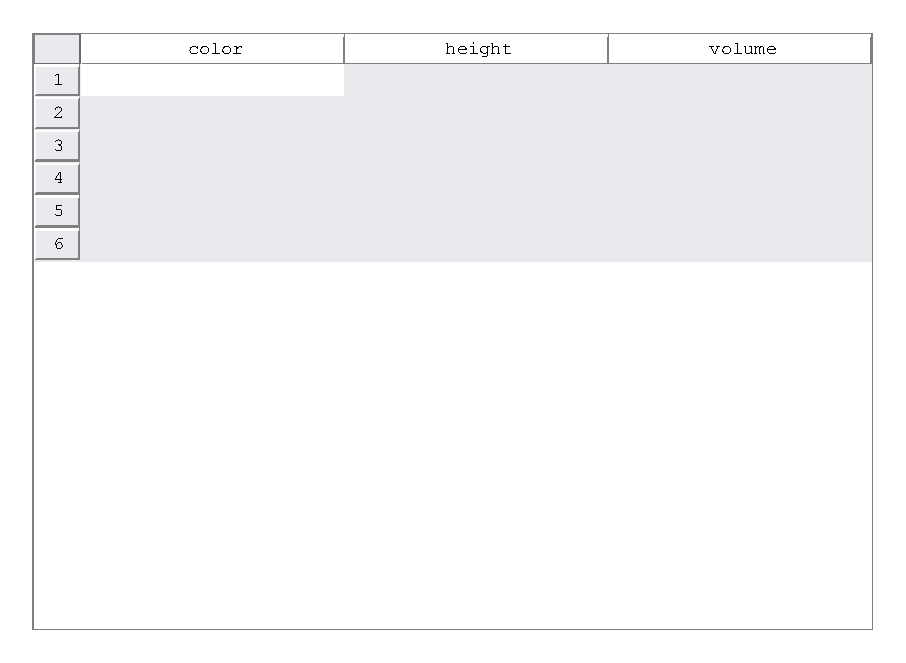
\includegraphics[trim={0 6cm 0 0},clip,width=1.2\textwidth]{../demo/geometricShape/report/figures/mtable}
\end{marginfigure}

Upon completion of the processing, the results of the last processing are displaying in the command window:

This display can be achieved by issuing the following command:
\begin{lstlisting}
geometricShape('display', 2, 'expose', '>', ...
	'mask', {[1 2] 0 1});
\end{lstlisting}
The exposition of relevant observations is important for efficient computational experimentation. \explanes provides many tools for this purpose, type \mcode{help expExpose} for quick reference. 


The command:
\begin{lstlisting}
geometricShape('display', 2, 'mask', {1 0 1},...
 'expose', {'t', 'obs', 3, 'sort', 1});
\end{lstlisting}

displays the volume (observation 3) of the step volume (2) for each cylinder of radius 2 sorted according to the first on a table (t). Red color indicates best performance, and blue ones, performances which have not been found statistically different from the best one. 
\marginnote{For this example, even if the blue cylinder is bigger than the blue one due to the uncertainty in the estimation of $\pi$, this difference is not significant, so the blue and red cylinders shall be considered of equivalent volume.}

\subsection{Report}

\begin{margintable}
\caption{\LaTeX output.}
\begin{tabular}{llc} 
color & height & volume \\ 
\hline 
blue & 2 &  26.12$\pm$9.30 \\ 
blue & 4 & 52.23$\pm$18.60 \\ 
blue & 6 & \textbf{\textcolor{red}{78.35$\pm$27.90}} \\ 
red & 2 &  24.61$\pm$7.54 \\ 
red & 4 & 49.23$\pm$15.07 \\ 
red & 6 & \textbf{73.84$\pm$22.61} \\ 
\end{tabular} 

\end{margintable}

The file \mcode{<shortExperimentName>Report.m}, that is \mcode{geshReport.m} in this example allows you to generate report that compile several expositions of observations: \LaTeX table (l), bar plot (b), and box plot (x).

\lstinputlisting[firstline=13, lastline=19]{../demo/geometricShape/geshReport.m}

\begin{marginfigure}
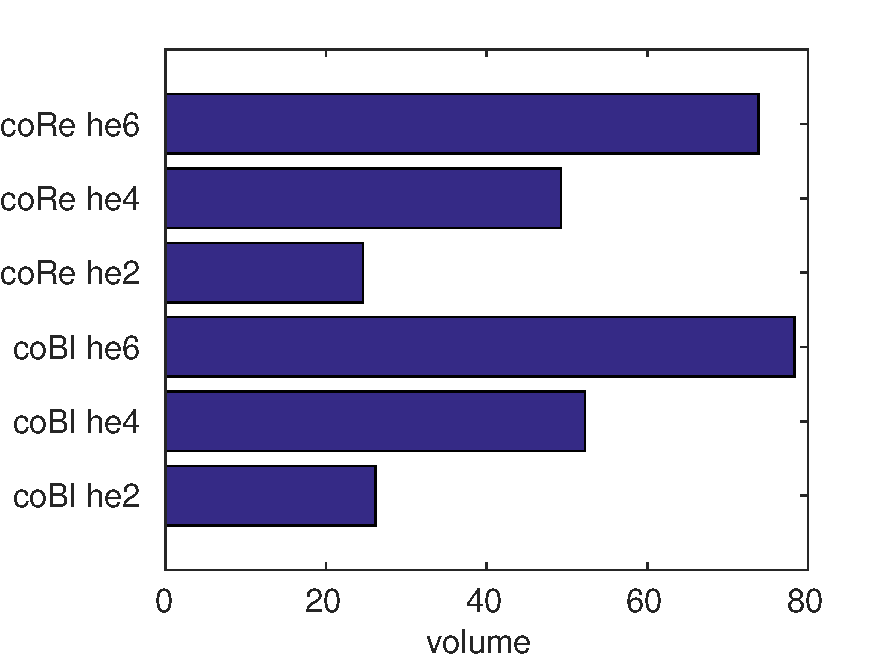
\includegraphics[width=\textwidth]{../demo/geometricShape/report/figures/geob}
\end{marginfigure}


\begin{marginfigure}
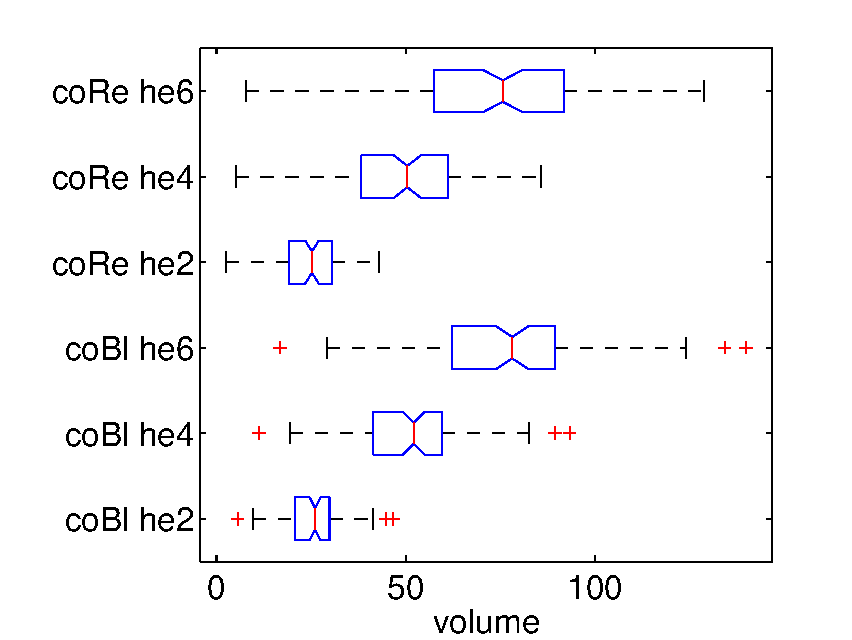
\includegraphics[width=\textwidth]{../demo/geometricShape/report/figures/geox}
\end{marginfigure}


Several reports can be handled for the same experiment using the key \mcode{'reportName'}, and if the name of the report contain the key \mcode{'Slides'}, a slide presentation layout is used. For example, the command:
\begin{lstlisting}
geometricShape('report', 'rcv', ...
  'reportName', 'presentationSlides');
\end{lstlisting} 
generates a report with base name \mcode{presentationSlides} in a slides presentation layout. For debug information about the compilation, please add the \mcode{'b'} flag to the \mcode{report} value.


\section{Architecture of an experiment}

An \explanes experiment has a specific directory architecture. 

\subsection{Code}

The main directory hosts the processing routines (named \mcode{codePath} in your configuration). It has the following files:
\begin{itemize}
\item \mcode{<projecName>}: main entry point of the experiment
\item \mcode{Factors}: text file encoding the factors of the experiment
\item \mcode{Init}: processed before any prcessing step
\item \mcode{Steps}: implement each processing units
\item \mcode{Report}: handle the generation of report that compile several types of expositions of observations
\end{itemize}

\subsection{Configuration}

The processing environment of the experiment can be controled with the files hosted in the directory \mcode{config}.

Almost every processing units of an \explanes experiment has access to a structure named \mcode{config} which is imported from a file which is specific to each user. This file is generated at the creation of the experiment from a user specific template file that can be found in \texttt{$\sim$/.\explanes}.

The syntax of this file allows the user to handle several configurations that depends on which machine the experiment is processed. For example, let us assume that the project handles 3 machines with different file architectures:
\begin{lstlisting}
machineNames  = {{'toto', 'yoyo'}, 'dodo', 'momo'}
codePath = {'~/code/geometricShape', '/lab/code/geometricShape}
\end{lstlisting}
If the experiment is processed on the machine \mcode{'toto'}, or \mcode{'yoyo'}, the \mcode{codePath} in the config structure is equal to \mcode{'~/code/geometricShape'}.  If the \mcode{codePath} has fewer entries than the one dedicated to the names of the machines, the last entry is chosen. Thus, if the experiment is processed on the machine \mcode{'dodo'}, or \mcode{'momo'}, the second entry is chosen, that is \mcode{'/lab/code/geometricShape'}.

Every entry of the configuration file can be overwritten at the command line call. For example:
\begin{lstlisting}
geometricShape('do', 0, 'sendMail', 1)
\end{lstlisting}
process every steps and sends an email at the end of the processing.

New entries can also be added and accessed in the processing files of the experiment for specific user usage:
\begin{lstlisting}
geometricShape('myEntry', 'toto')
\end{lstlisting}
outputs:
\begin{lstlisting}
Warning. The command line parameter myEntry is not found
 in the Config file. Setting anyway.
\end{lstlisting}


\subsection{Data}

Access to input data is handled in the configuration file with the entry \mcode{inputPath}. Processing data is handled with the entry \mcode{dataPath}. Before processing any step, a directory is created with the name of the step and processing data generated by this step is stored here.

Observations are usually of smaller size. As such it may useful to store them in a different location such as a cloud filesystem. The \mcode{obsPath} stores the observation data in the same directory architecture. If left empty, the \mcode{obsPath} is set equal to \mcode{dataPath}.


\subsection{Report}

The report directory stores expositions of observations in many flavors.

\begin{itemize}
\item \textbf{\mcode{report/}}: contains editable \LaTeX files, one for each \mcode{reportName} (default to \mcode{<projectName>.tex}) and BibTex file that can be edited and processed in a standard fashion. Expositions of observations are added to the \LaTeX file prior compilation at the location of the flag \mcode{expLanesInsertionFlag}.
\item \textbf{\mcode{report/figures}}: when the \mcode{'save'} parameter is added to a visual exposition, the resulting figure is stored in several formats (\mcode{.fig} Matlab Figure, \mcode{.eps}, \mcode{.png}, and \mcode{.pdf}). The numerical data is also made available in a \mcode{.mat} file. 
\item \textbf{\mcode{report/reports}}: contains the generated reports with the following naming : \mcode{<reportName><userName><date>.pdf}. The data of every expositions of the corresponding report is made available in a \mcode{.mat} file.
\item \textbf{\mcode{report/tables}}:  when the \mcode{'save'} parameter is added to a table exposition (\mcode{'t'} or \mcode{'l'}), the resulting table is stored in several formats (\LaTeX floating table, \LaTeX tabulary array, \mcode{.csv} file. The numerical data is also made available in a \mcode{.mat} file.
\item \textbf{\mcode{report/tex}}: this directory is used for internal \explanes usage. Please do not edit any files in it, as they may be deleted.
\end{itemize}


\section{Configuration of an experiment}

An \explanes experiment can be controlled by editing the configuration file or overloading it with command line settings. Each of those parameters can further be accessed at run time through the variable \mcode{config}.

\subsection{User}

\begin{itemize}
\item \textbf{emailAddress}: email address ticked when processing is done server side (leave empty for no mailing service), can be a cell array of email adresses
\item \textbf{completeName}: complete name of user
\end{itemize}

\subsection{Project}

\begin{itemize}
\item \textbf{probe}: probe tools (1), paths (2), and hosts (3), or all (0)
\item \textbf{generateRootFile}: regenerate the root file of the experiment (use of newer versions of the expLanes lib may reguired it)
\item \textbf{addFactor}: add a factor to the experiment. Format of the request: {'name', 'modalities', 'steps', 'selector', defaultModalityId, rankInFactorFile}
\item \textbf{removeFactor}: remove a factor of the experiment. Format of the request: {rankInFactorFile, defaultModalityId}
\item \textbf{addStep}: add a step to the experiment. Format of the request: {'name', rank}
\item \textbf{removeStep}: remove a given step of the experiment. Format of the request: rank
\end{itemize}

\subsection{Hostnames and Paths}



\begin{itemize}
\item \textbf{machineNames}: names of the machines as a cell array of 1) string or 2) cell array of strings
\item \textbf{inputPath}: path to input data (usually accessed read only)
\item \textbf{codePath}: path to the code repository of the experiment
\item \textbf{dataPath}: path to the data repository of the experiment  (structured with one directory per step)
\item \textbf{obsPath}: path to the data repository of the experiment for observation data (same as dataPath if left blank)
\item \textbf{backupPath}: path to backup of transferred data
\item \textbf{bundlePath}: path to export bundles
\item \textbf{matlabPath}: path to the directory of the Matlab binary 
\item \textbf{toolPath}: path to Unix tools (pdflatex, rsync, ssh, screen)
\end{itemize}

Every path can be a cell array of string. In this case, the path is selected in the cell array according to the rank of the host in the machineNames field.

\subsection{Code}

\begin{itemize}
\item \textbf{dependencies}: code dependencies to load and export as a cell array of strings with paths to the dependencies
\item \textbf{localDependencies}: dependencies (including expLanes) can be part of the experiment in a dependencies directory: 0 do not use local versions, 1 use local versions, 2 update local versions
\item \textbf{codeVersion}: version tag of the code of the experiment
\end{itemize}

\subsection{Computing}

\begin{itemize}
\item \textbf{do}: processing steps to execute: -1 none, 0 all, >0 processing step by numeric id
\item \textbf{resume}: do not perform computation if data and obs files with runID>resume are already there
\item \textbf{parallel}: use parallel processing, if |parallel|>1 specify the number of cores, if array set at step level, if >0 parallelize settings, if <0 parallelize within each setting (the code of the step shall use parfor or the like), can be a numeric value for all processing steps or an array of numeric value, one per step
\item \textbf{mask}: factor mask: cell array defining the modalities to be set for the factors (0 do all, 1 first modality, [1 3] first and third modality), can be a cell array of cell array

\item \textbf{design}: use a canonical experimental design: assume cell array of {[factors as numericIds], number of values per factor (0 complete set of values), type of plan as string 'f' (factorial) or 'o' (one factor at a time), [seed as a vector of index of factor]}
\item \textbf{dummy}:  dummy mode: allow for short computations to dry run the experiment. Set as a numeric value. 0: no dummy mode, >1 generate stored data and observations flagged with the numeric value
\item \textbf{setRandomSeed}: set the random seed at init for replicability purposes, 0 do not set, >0 set to value.
\item \textbf{host}: host index to run the experiment: 0: seek by hostName, >0: server mode, <0: local mode, 2.1 means the first host of the second compound (cell array)
\item \textbf{log}: log level (set to 0 for no log)
\item \textbf{progress}: show processing progress 0: none, 1: garphical bar if on local mode, 2: verbose output, 3: liminar output
\item \textbf{exitMatlab}: exit matlab at the end of the computation
\item \textbf{recordTiming}: show timing observations
\end{itemize}

\subsection{Data}

\begin{itemize}
\item \textbf{encodingVersion}: encoding type of mat files (doc save for specs)
\item \textbf{store}: perform computation to be stored: (1, 0) load data of previous step, (-1, 0) load data result of the current step
\item \textbf{retrieve}: retrieve needed data server side: -1 no retrieval, 0 global scan of every hosts, >0 hostId
\item \textbf{namingConventionForFiles}: naming convention for data files: long (complete naming, may lead to too long file names), short (abbreviated naming, may also lead to too long file names), hash (hash based naming, compact but may lead to naming clashes)
\item \textbf{bundle}: generate bundle of elements designated as a string with tokens separated by white spaces: 'c' (code), 'd' (dependencies), 'i' (input), 1 (output data of step 1), 1d (stored data of step 1 only), 1o (observations of step 1 only) 
\item \textbf{sync}: sync data across machines specified as a cell array with: elements (as in bundle), optional host as numeric id (1.2 means the second host of the first group of machines, default to 2), direction 'd' (download from server to local host, default), 'u' (upload from host to server). Provided with the elements as string, the command default to server 2 in download mode.
\item \textbf{clean}: clean explanes directories and project data repositories. As string id : t (expLanes temporary directory), b (experiment backup directory), k (all steps directories while keeping reachable settings), 1 (output data of step 1), 1d (remove stored data of step 1 only), 1o (observations of step 1 only). As numeric id (clean the corresponding step directory, 0 means all directories) 
\item \textbf{branchStep}:  specify at which step the branching (if any) is effective (default 0)
\end{itemize}

\subsection{Exposition}

\begin{itemize}
\item \textbf{display}: step for which to display observations: -1 none, 0 last processed step if any, >0 specific step
\item \textbf{expose}: specify default display of observations (>: prompt, t: table, p:plot)
\item \textbf{tableDigitPrecision}: mantissa precision for the display of observations
\item \textbf{displayFontSize}: font size for the display of observations in figures
\end{itemize}

\subsection{Report}

\begin{itemize}
\item \textbf{report}: generate report: combination of r (run report), c (LaTeX compilation), and d (debug output)
\item \textbf{reportName}: type of report: empty (default), if containing the word <slides> or <Slides>,  beamer presentation mode is used
\item \textbf{latexDocumentClass}: style of LaTeX document (warning: this parameter is taken into account only at the creation of the LaTeX report file)
\item \textbf{pdfViewer}: path to the pdf viewer (if left empty, expLanes try to locate it automatically)
\item \textbf{significanceThreshold}: threshold for statistical significance testing
\item \textbf{showFactorsInReport}: show the factors graph in the report: 0, no display, 1 compact display, 2 alos show stored data, 3 also show observations, 4 also show stored data and observations (if negative only generate the figure for latter inclusion)
\item \textbf{factorDisplayStyle}:  style of the factor graph: 0 no propagation of factors, 1 propagation of factors, 2 propagation of factors with an "all steps" node
\item \textbf{figureCopyPath}: path where saved figures are copied outside the expLanes project
\item \textbf{tableCopyPath}: path where saved tables are copied outside the expLanes project
\end{itemize}

\subsection{Miscellaneous}

\begin{itemize}
\item \textbf{useExpCodeSmtp}: usage of default expcode smtp. If set to 0 assume availability of local stmp server with complete credentials
\item \textbf{sendMail}: send email: -2, server mode, email at start and end, -1 server mode, email at end only, 0, no email ever, 1 one email at end, 2 email at start and end
\end{itemize}

\section{Exposition of observations}

To generate Tables, Figures that can be saved or embedded in your reports, the main function to use is:

\mcode{config = expExpose(config, '<typeOfExposition>', <parameters>);}

The type of exposition specify the style of rendering. Several predefined styles are available and custom ones can easily be built. Parameters customizes the rendering and are defined as pair of string / value.

\textbf{Important}: as \explanes do not use global variables, the state of the experiment is entirely stored in the variable \mcode{config}. Therefore, this variable has to be propagated trough each of the exposition calls.

\subsection{Available expositions}

Available expositions are:
\begin{itemize}
\item \textbf{>}: redirect the observations to the command prompt
\item \textbf{l}: generate a \LaTeX table
\item \textbf{t}: Matlab table
\item \textbf{b}: bar plot
\item \textbf{p}: line plot
\item \textbf{s}: scatter plot with up to 4 observations respectively mapped to the x-axis, the y-axis, the point size and the color
\item \textbf{x}: box plot
\item \textbf{a}: anova display
\item \textbf{i}: image display
\end{itemize}

\subsection{Custom exposition}

Let us assume that you need a custom way of displaying observations. You can do so:

\mcode{config = expExpose('custom');}

At the first call, the user is prompted:

\texttt{Unable to find the function exposeCustom in your path. This function is needed to display the observations with the Custom type of display. \\
Do you want to create it ? Y/N [Y]:}

After acknowledgment, the script if generated in the \mcode{codePath}. This function has the following signature:

\mcode{config = exposeCustom(config, data, p)}

where,
\begin{itemize}
\item \textbf{config}: contains the \explanes configuration state                  
\item \textbf{data}: contains the observations as a struct array                  
\item \textbf{p}: contains the exposition parameters   
\end{itemize}

\subsection{Parameters}

Parameters customizes the rendering and are defined as pair of string / value.

\begin{itemize}
\item \textbf{addSpecification}: add display specification to plot directive
    	as ('parameter' / value) pairs;
           value can be a cell array, in this case the cell array is split
           across plot items                 
\item \textbf{addSettingSpecification}:  add display specification to plot;
           directive relative to specific settings as ('parameter' / value) pairs,
           value have to be a cell array which is split
           across plot items which corresponds to the settings                
\item \textbf{caption}: caption of display as string;
    	symbol + gets replaced by a compact description of the setting  
\item \textbf{color}: color of line;
           1: default set of colors
           0: black
           {'r', ...}: user defined set of colors                 
\item \textbf{compactLabels}: shorten labels by removing common substrings
           (default 0)                 
\item \textbf{data}: specify data to be stored (default empty)  
\item \textbf{expand}: name or index of the factor to expand                 
\item \textbf{fontSize}:  set the font size of \LaTeX tables (default 'normal')                
\item \textbf{highlight}:  highlight settings that are not significantly
    	different from the best performing setting;
       -1: no variance,
    	0: variance for all observations,
    	[1, 3]: variance for the first and third observations 
\item \textbf{highlightStyle}:  type of highlighting;
        'best': highlight best and equivalents (default),
        'Best': highlight only the best,
        'better': highlight only the best if significantly better than
           the others,
        'Better': highlight only the best if significantly better than
           the others and show only this one                
\item \textbf{highlightColor}: use color to show highlights (default 1), -1 do
       not use * to display the best performing one                 
\item \textbf{integrate}:  factor(s) to integrate by summation 
\item \textbf{label}: \LaTeX label of display as string (equal to the name if left empty)             
\item \textbf{legendLocation}: location of the legend (default 'BestOutSide', doc legend for more options)                 
\item \textbf{marker}:  specification of markers for line plot;
           1: Matlab default set of markers (default),
           0: no markers,
           {'', ...}: user defined cell array of markers 
\item \textbf{mask}:    selection of the settings to be displayed              
\item \textbf{mergeDisplay}: concatenate current display with the previous one;
        '': no merge (default),
        'h': horizontal concatenation,
        'v': vertical concatenation                 
\item \textbf{multipage}:   activate the multipage setting to the \LaTeX table 
\item \textbf{name}:   name of exported file as string; 
    	symbol + gets replaced by a compact description of the setting              
\item \textbf{number}:  add a line number for each setting in tables                
\item \textbf{noFactor}:  remove setting factors 
\item \textbf{noObservation}: remove observations                 
\item \textbf{obs}: name(s) or index(es) of the observations to display                 
\item \textbf{orderFactor}:   numeric array specifying the ordering of the factors
\item \textbf{orderSetting}:    numeric array specifying the ordering of the settings              
\item \textbf{orientation}:  orientation of display;
    	'v': vertical (default),
    	'h': horizontal,
       'i': as second letter invert the table for prompt and latex
           display                
\item \textbf{percent}: display observations in percent;
    	selector is the same as 'highlight'  
\item \textbf{plotCommand}:  set of commands executed after the plotting
       directives as a cell array of commands                  
\item \textbf{plotAxisProperties}: set of command setting the current axis after plotting
       directives as a cell array of couple property / value (see axis properties in Matlab documentation)  
\item \textbf{precision}:  mantissa precision of data as numeric value or array;
           -1: take value of \mcode{config} parameter tableDigitPrecision (default),
           0: no mantissa                  
\item \textbf{put}: specify display output;
    	0: otuput to command prompt,
    	1: output to figure,
    	2: output to \LaTeX 
\item \textbf{report}:  include the current exposition in the report;
       0: do not include (default for Matlab tables),  
       1: include (default for other displays)                   
\item \textbf{rotateAxis}: rotate X axis labels (in degrees)   
\item \textbf{show}: display;
        'data': actual observations (default),
        'rank': ranking among settings,
        'best': select best approaches,
        'Best': select the significantly best approach (if any)                 
\item \textbf{save}: save the display;
    	0: no saving,
    	1: save to a file with the name of the display as filename
    	'name': save to a file with 'name' as filename
\item \textbf{shortObservations}: compact observation names                 
\item \textbf{shortFactors}: compact factor names  
\item \textbf{showMissingSetting}:  show missing settings (default 0)                
\item \textbf{sort}:   sort settings acording to the specified set of observations if
        positive or to the specified set of factors if negative
\item \textbf{step}: show observations the specified processing step as name or
    index (default last step)                 
\item \textbf{title}: title of display as string,
    	symbol + gets replaced by a compact description of the setting  
\item \textbf{total}:  display average  or summed values for observations;
        'v', 'V': vertical with (v) or without (V) display of settings,
        'h', 'H': horizontal with (h) or without (H) display of settings                
\item \textbf{variance}:   display variance;
    	selector is the same as 'highlight',
\item \textbf{visible}: show the figure (default 1 except in save mode)                    
\end{itemize}

\section{Advanced usage}

\subsection{Branching experiments}

Experimental research most of the time involves the implementation of many solution that will potentially improve things for a given step of the experiment. Finding the correct way to do it requires a lot of trials that may lead to code burden.

In order to keep a root project clean, and not to replicate the code and data and of this root project in another more experimental project, \explanes allows us to create a branch experiment that accesses the data generated by the root experiment.

Let us assume that we want to create a new way of computing the volume of our geometric shapes. We can do so by creating a branch experiment:

\mcode{expBranch('branchGeometricShape', <pathToGeometricShape>, 2)}

The last parameter specifies at which step the branching is done, in this case at step 2.
The new experiment must keep the same factors up to the step before the branching step (in our case step 1).

The merge of the new solution to the root experiment must be done by hand.

\subsection{Design of factorial exploration}



%\section{Best practices} \label{sec:best}
%
%factorial design
%
%multi way anova
%
%main concepts
%
%experiment statement
%
%factors, modalities
%
%processing
%
%processing steps
%
%parallelization, independance, sequentiality
%
%factorial tree
%
%data / observations
%
%Main steps
%
%definition
%computation
%mining
%reporting
%
%distant computing
%data retrieval

\section{Recommended readings}

\begin{itemize}

\item \textbf{Getting it right}: R\&D Methods for Science and Engineering, Peter Bock, Academic Press

\item \textbf{The Visual Display of Quantitative Information} Edward R. Tufte

\end{itemize}









\bibliographystyle{plain}
\bibliography{references}

\end{document}